\chapter{Game metrics plots}
\label{all_game_metrics}

This chapter contains all the metrics computed for Tricolor, in addition to the ones presented in Chapter~\ref{game_metrics} and Chapter~\ref{perf_analysis_of_agents}.

These are the following metrics, as well as their definitions and sources of inspiration:
\begin{itemize}
    \item \textit{Duration} -- measures the duration of a game in turns. A turn is equivalent to a move made by any of the 2 players.
    
    Source: inspired from~\cite{browne2010evolutionary} and~\cite{shannon1950chess2}.
    
    \item \textit{Branching Factor} -- measures how many possible actions any player can choose from, on average, during their turn.
    
    Source: inspired from~\cite{shannon1950chess2}.
    
    \item \textit{Decision Moves} -- measures what percentage of the moves made by any player during a game aren’t forced. A move isn’t forced if the player can choose between at least 2 actions during their turn.
    
    Source: inspired from~\cite{ludii_concepts}.
    
    \item \textit{State Repetition} -- measures how many times the same states are repeated during a game. A state is repeated whenever the Tricolor board reaches a position equivalent to a previous one during the same game. Two positions are equivalent if they contain the same pieces on the same tiles, controlled by the same players, and with the same player to move.
    
    Source: inspired from the~\cite{ludii_concepts}.
    
    \item \textit{Decision Factor} -- measures how many possible actions any player can choose from, on average, during their turn, ignoring turns where only one move is possible.
    
    Source: inspired from~\cite{ludii_concepts}.
    
    \item \textit{Board Sites Occupied} -- measures how many board tiles were occupied by any player at least once during the game. Initially, both players occupy 18 tiles each, so 36 tiles in total. The board has a total of 61 tiles, so, for each game, the value of this metric is between 36 and 61.
    
    Source: inspired from~\cite{ludii_concepts}.
    
    \item \textit{Move Distance} -- measures the average distance traveled by pieces when they move around the board during a game. In Tricolor, a stack of pieces can move at a distance of 1, 2 or 3 tiles, depending on the number of pieces on the stack (see Game Rules \ref{game_rules}).
    
    Source: inspired from~\cite{ludii_concepts}.
    
    \item \textit{Piece Number} -- measures the average number of pieces on the board during a game. Players start with 18 pieces each, so there are 36 pieces in total initially on the board.
    
    Source: inspired from~\cite{ludii_concepts}.
    
    \item \textit{Game Outcome} -- measures the percentage of games won by Player 1 (White), Player 2 (Black) and draws.
    
    Source: inspired from~\cite{browne2010evolutionary}.
    
    \item \textit{Narrowness} -- measures the average narrowness of all the turns of a game. The narrowness of a turn represents the number of considerable actions a player can choose from during that turn. An action is considerable if it improves or maintains the current score of the position for the player to move.
    
    Source: inspired from~\cite{browne2008recombination} and~\cite{ludii_concepts}.
    
    \item \textit{Decisiveness} -- measures the proportion of the game completed before the eventual winner establishes a decisive advantage that is maintained until the end of the game. This metric is only computed when a game has a winning player, so draws a discarded.
    
    Source: inspired from~\cite{browne2008recombination}.
    
    \item \textit{Lead Change} -- measures the average number of possible actions during a turn that change the leader of the game. The leader of the game is the player who has a positional advantage.
    
    Source: inspired from~\cite{ludii_concepts}.
    
    \item \textit{Stability} -- measures the percentage of moves in a game that changed the leader. Its purpose is to assess how stable games are.
    
    Source: inspired from~\cite{browne2010evolutionary} (called \textit{Uncertainty} in the paper) and~\cite{ludii_concepts}.
    
    \item \textit{Drama} -- measures the average change in position evaluation scores throughout a game. Its purpose is to see how big the jumps are on average between consecutive turns during a game in terms of position evaluation. 
    
    Source: inspired from~\cite{browne2010evolutionary}, ~\cite{browne2008recombination} and~\cite{ludii_concepts}.
\end{itemize}

\section{Random Agent vs Random Agent simulations}

\newpage %%%%%%%%%%%%%%%%%%

\begin{figure}[p]
\centering

% Row 1
\begin{minipage}{0.48\linewidth}
    \centering
    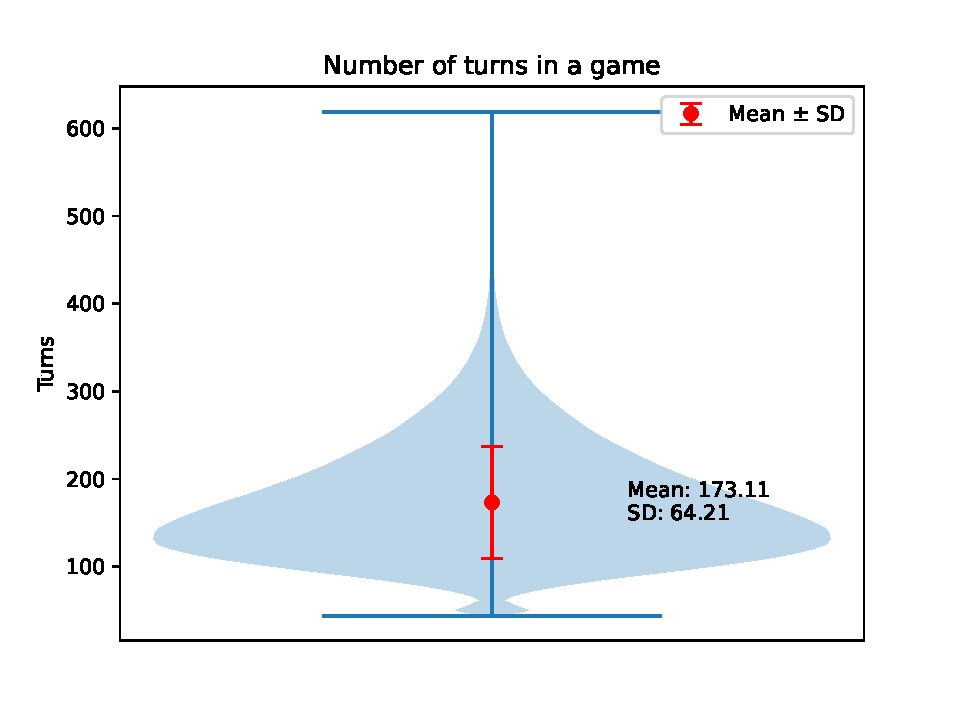
\includegraphics[width=\linewidth]{game_metrics/images/total_turns.pdf}
\end{minipage}
\hfill
\begin{minipage}{0.48\linewidth}
    \centering
    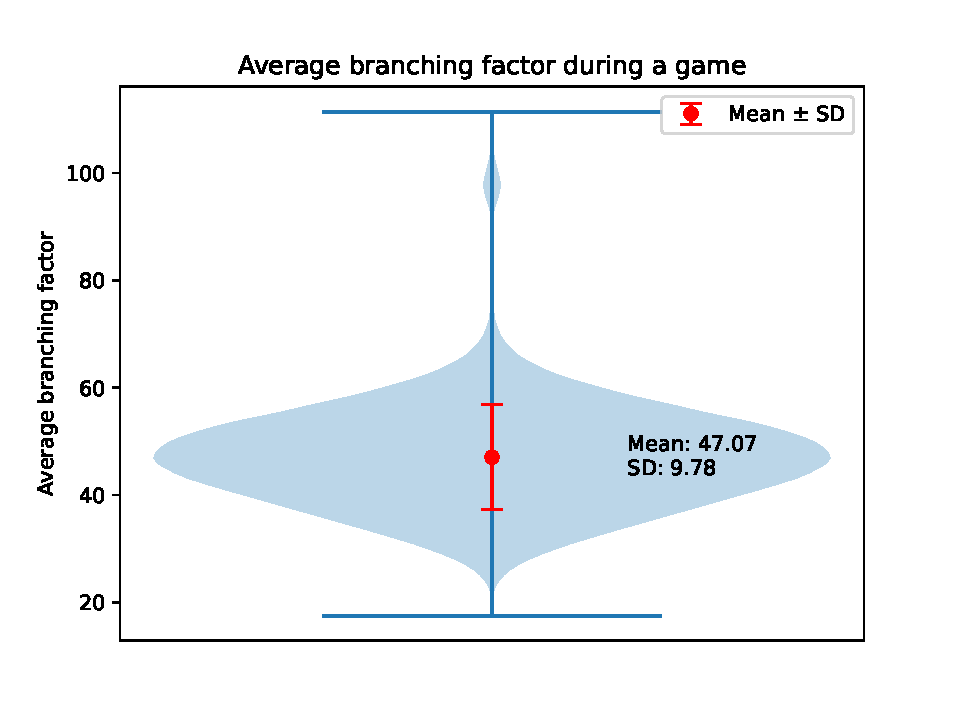
\includegraphics[width=\linewidth]{game_metrics/images/total_branches.pdf}
\end{minipage}

\vspace{0.5cm}

% Row 2
\begin{minipage}{0.48\linewidth}
    \centering
    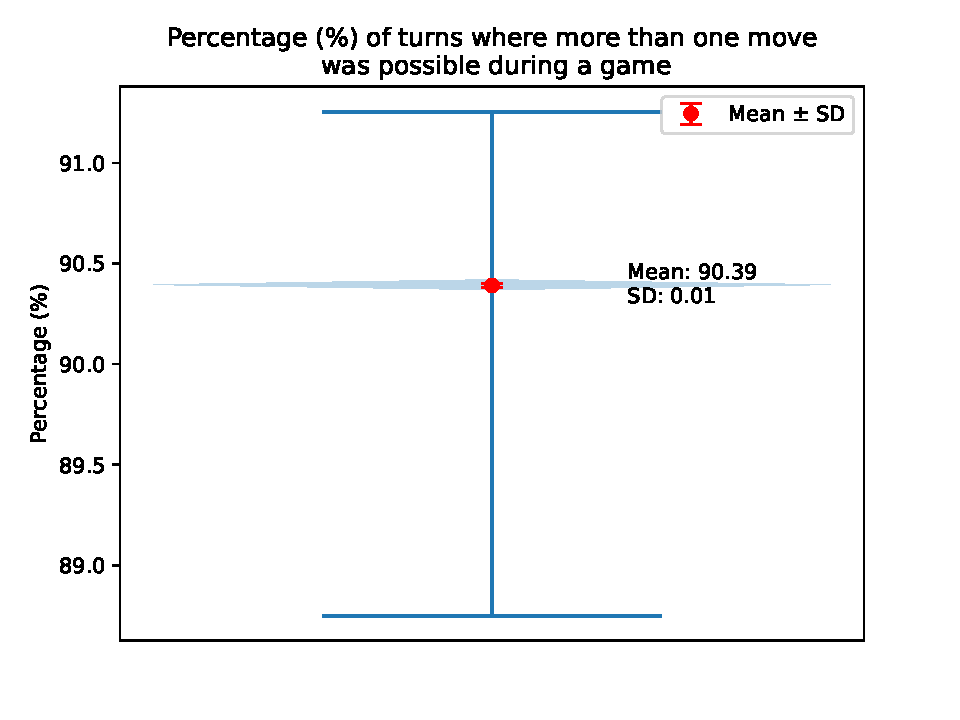
\includegraphics[width=\linewidth]{game_metrics/images/total_more_than_one_move.pdf}
\end{minipage}
\hfill
\begin{minipage}{0.48\linewidth}
    \centering
    
\includegraphics[width=\linewidth]{game_metrics/images/total_repeated_states.pdf}
\end{minipage}

% Row 3
\begin{minipage}{0.48\linewidth}
    \centering
    
\includegraphics[width=\linewidth]{game_metrics/images/total_decision_factors.pdf}
\end{minipage}
\hfill
\begin{minipage}{0.48\linewidth}
    \centering
    
\includegraphics[width=\linewidth]{game_metrics/images/total_occupied_tiles.pdf}
\end{minipage}

% Row 4
\begin{minipage}{0.48\linewidth}
    \centering
    
\includegraphics[width=\linewidth]{game_metrics/images/total_distance.pdf}
\end{minipage}
\hfill
\begin{minipage}{0.48\linewidth}
    \centering
    
\includegraphics[width=\linewidth]{game_metrics/images/total_number_of_pieces.pdf}
\end{minipage}

\caption{}
\label{fig:allplots1}
\end{figure}

\newpage %%%%%%%%%%%%%%%%%%%%%%%%%%%%%%%%%%%

\begin{figure}[p]
\centering

% Row 1
\begin{minipage}{0.48\linewidth}
    \centering
    
\includegraphics[width=\linewidth]{game_metrics/images/winrates.pdf}
\end{minipage}
\hfill
\begin{minipage}{0.48\linewidth}
    \centering
    
\includegraphics[width=\linewidth]{game_metrics/images/total_narrowness.pdf}
\end{minipage}

\vspace{0.5cm}

% Row 2
\begin{minipage}{0.48\linewidth}
    \centering
    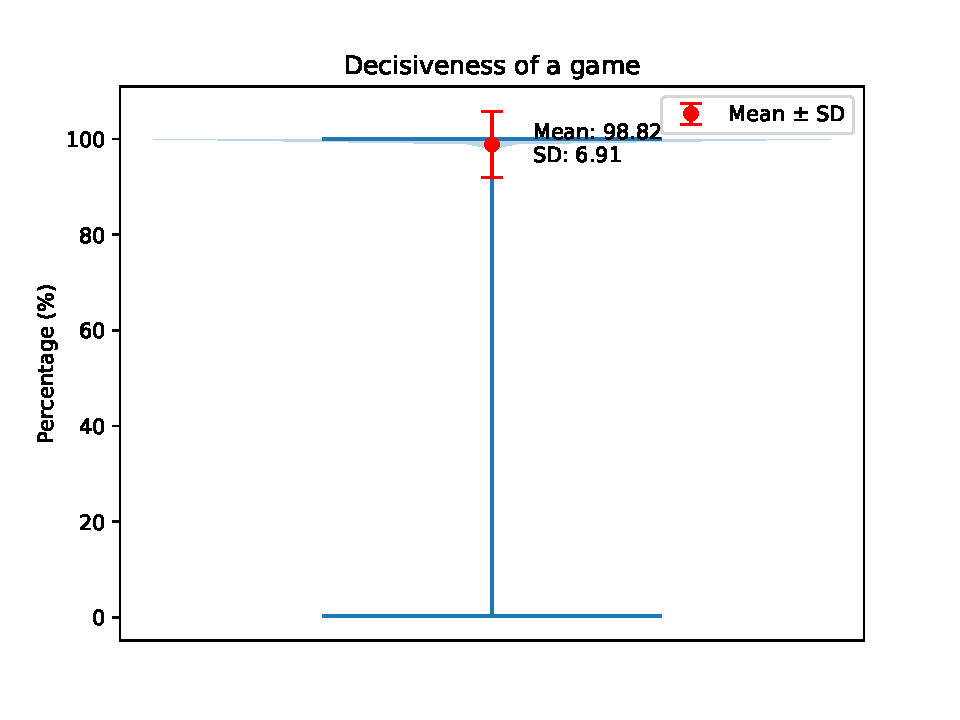
\includegraphics[width=\linewidth]{game_metrics/images/decisiveness.pdf}
\end{minipage}
\hfill
\begin{minipage}{0.48\linewidth}
    \centering
    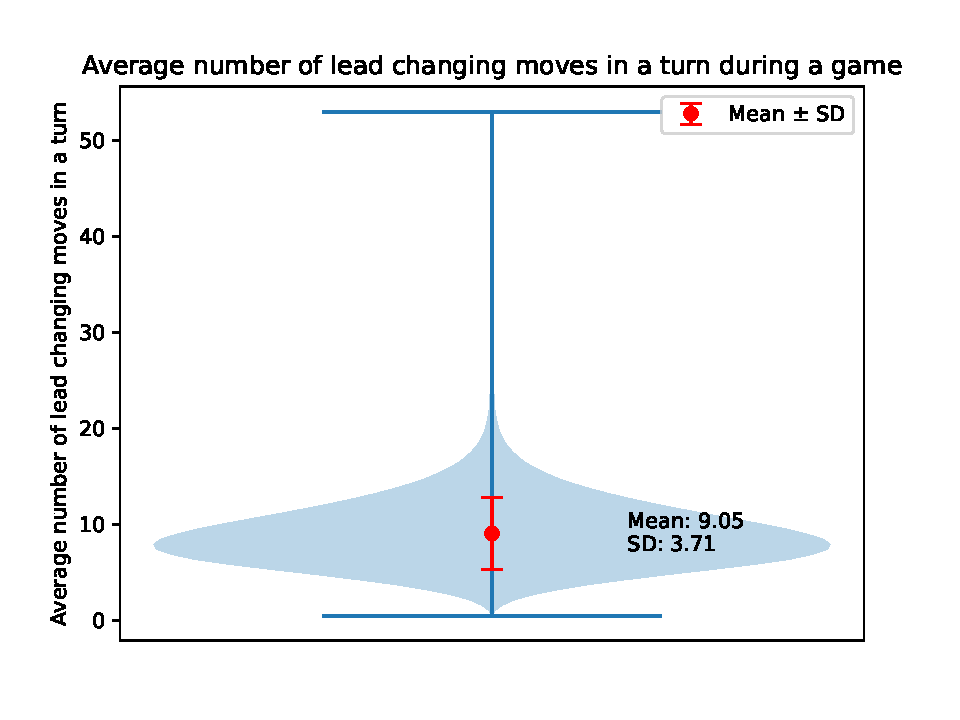
\includegraphics[width=\linewidth]{game_metrics/images/total_lead_change_moves.pdf}
\end{minipage}

% Row 3
\begin{minipage}{0.48\linewidth}
    \centering
    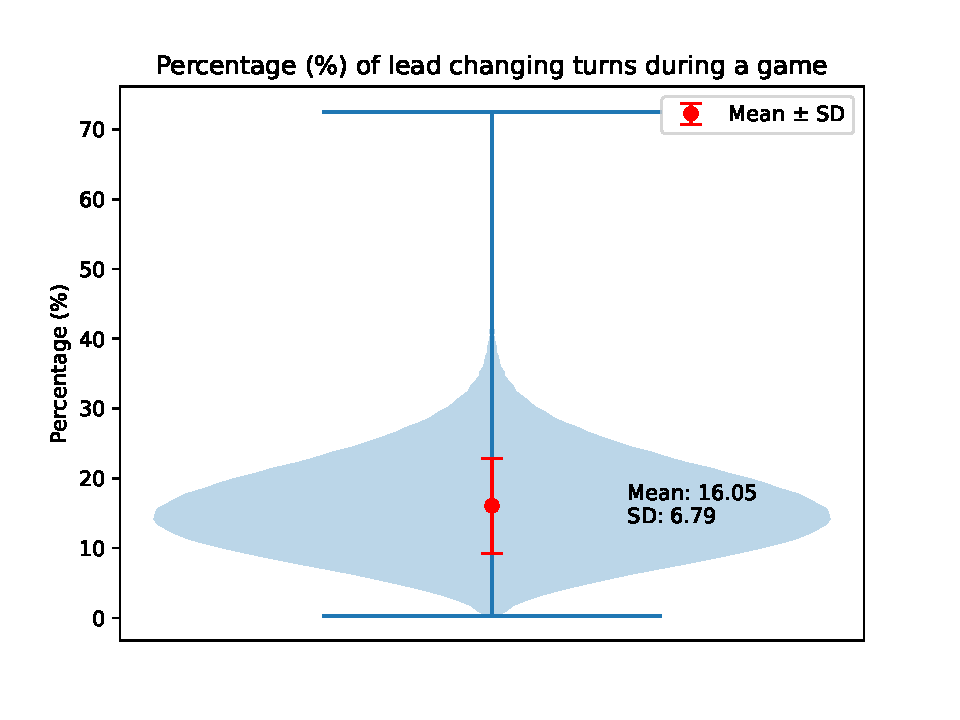
\includegraphics[width=\linewidth]{game_metrics/images/total_lead_change_actions.pdf}
\end{minipage}
\hfill
\begin{minipage}{0.48\linewidth}
    \centering
    
\includegraphics[width=\linewidth]{game_metrics/images/total_drama.pdf}
\end{minipage}

% Row 4
\begin{minipage}{0.48\linewidth}
    \centering
    
\includegraphics[width=\linewidth]{game_metrics/images/game_evaluation_1.pdf}
\end{minipage}
\hfill
\begin{minipage}{0.48\linewidth}
    \centering
    
\includegraphics[width=\linewidth]{game_metrics/images/game_evaluation_2.pdf}
\end{minipage}

\caption{}
\label{fig:allplots}
\end{figure}

\section{Alpha-Beta Agent vs MCTS Agent simulations}

\newpage %%%%%%%%%%%%%%%%%%%%%

\begin{figure}[p]
\centering

% Row 1
\begin{minipage}{0.48\linewidth}
    \centering
    
\includegraphics[width=\linewidth]{all_game_metrics/images/alphabeta_vs_mcts/total_turns.pdf}
\end{minipage}
\hfill
\begin{minipage}{0.48\linewidth}
    \centering
    
\includegraphics[width=\linewidth]{all_game_metrics/images/alphabeta_vs_mcts/total_branches.pdf}
\end{minipage}

\vspace{0.5cm}

% Row 2
\begin{minipage}{0.48\linewidth}
    \centering
    
\includegraphics[width=\linewidth]{all_game_metrics/images/alphabeta_vs_mcts/total_more_than_one_move.pdf}
\end{minipage}
\hfill
\begin{minipage}{0.48\linewidth}
    \centering
    
\includegraphics[width=\linewidth]{all_game_metrics/images/alphabeta_vs_mcts/total_repeated_states.pdf}
\end{minipage}

% Row 3
\begin{minipage}{0.48\linewidth}
    \centering
    
\includegraphics[width=\linewidth]{all_game_metrics/images/alphabeta_vs_mcts/total_decision_factors.pdf}
\end{minipage}
\hfill
\begin{minipage}{0.48\linewidth}
    \centering
    
\includegraphics[width=\linewidth]{all_game_metrics/images/alphabeta_vs_mcts/total_occupied_tiles.pdf}
\end{minipage}

% Row 4
\begin{minipage}{0.48\linewidth}
    \centering
    
\includegraphics[width=\linewidth]{all_game_metrics/images/alphabeta_vs_mcts/total_distance.pdf}
\end{minipage}
\hfill
\begin{minipage}{0.48\linewidth}
    \centering
    
\includegraphics[width=\linewidth]{all_game_metrics/images/alphabeta_vs_mcts/total_number_of_pieces.pdf}
\end{minipage}

\caption{}
\label{fig:allplots1}
\end{figure}

\newpage %%%%%%%%%%%%%%%%%%%%%%%%%%%%%%%%%%%

\begin{figure}[p]
\centering

% Row 1
\begin{minipage}{0.48\linewidth}
    \centering
    
\includegraphics[width=\linewidth]{all_game_metrics/images/alphabeta_vs_mcts/winrates.pdf}
\end{minipage}
\hfill
\begin{minipage}{0.48\linewidth}
    \centering
    
\includegraphics[width=\linewidth]{all_game_metrics/images/alphabeta_vs_mcts/total_narrowness.pdf}
\end{minipage}

\vspace{0.5cm}

% Row 2
\begin{minipage}{0.48\linewidth}
    \centering
    
\includegraphics[width=\linewidth]{all_game_metrics/images/alphabeta_vs_mcts/decisiveness.pdf}
\end{minipage}
\hfill
\begin{minipage}{0.48\linewidth}
    \centering
    
\includegraphics[width=\linewidth]{all_game_metrics/images/alphabeta_vs_mcts/total_lead_change_moves.pdf}
\end{minipage}

% Row 3
\begin{minipage}{0.48\linewidth}
    \centering
    
\includegraphics[width=\linewidth]{all_game_metrics/images/alphabeta_vs_mcts/total_lead_change_actions.pdf}
\end{minipage}
\hfill
\begin{minipage}{0.48\linewidth}
    \centering
    
\includegraphics[width=\linewidth]{all_game_metrics/images/alphabeta_vs_mcts/total_drama.pdf}
\end{minipage}

% Row 4
\begin{minipage}{0.48\linewidth}
    \centering
    
\includegraphics[width=\linewidth]{all_game_metrics/images/alphabeta_vs_mcts/game_evaluation_1.pdf}
\end{minipage}
\hfill
\begin{minipage}{0.48\linewidth}
    \centering
    
\includegraphics[width=\linewidth]{all_game_metrics/images/alphabeta_vs_mcts/game_evaluation_2.pdf}
\end{minipage}

\caption{}
\label{fig:allplots}
\end{figure}